\section{Extrinsic Parameters}
\begin{figure}[h!]
    \centering
    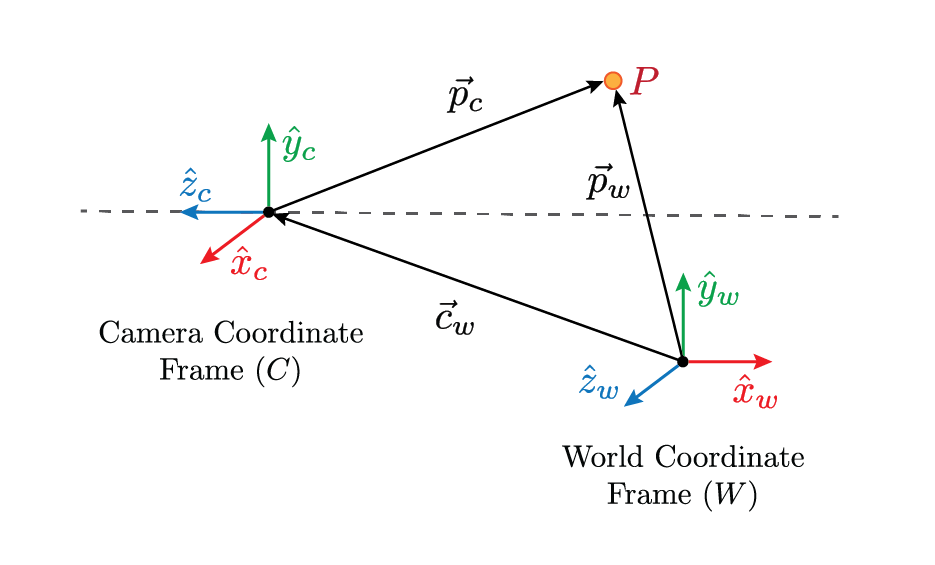
\includegraphics[width=0.9\textwidth]{figures/coord_transform}
    \caption{Coordinate transformation.}
\end{figure}

\begin{equation}
    \vec{p}_c = M_{ext}\vec{p}_w
\end{equation}

\begin{equation}
    R =
    \begin{bmatrix}
        r_{11} & r_{12} & r_{13} \\
        r_{21} & r_{22} & r_{23} \\
        r_{31} & r_{32} & r_{33}
    \end{bmatrix}
\end{equation}


\begin{subequations} \label{eqn:main}
    \begin{alignat}{2}
        \vec{p}_c & = R(\vec{p}_w-\vec{c}_w) \label{subeqn:a} \\
                  & = R\vec{p}_w -R\vec{c}_w \label{subeqn:b}
    \end{alignat}
\end{subequations}


\begin{gather}
    \vec{p}_c = R\vec{p}_w + \vec{t} \\
    \begin{bmatrix}
        x_c \\ y_c \\ z_c
    \end{bmatrix}
    =
    \begin{bmatrix}
        r_{11} & r_{12} & r_{13} \\
        r_{21} & r_{22} & r_{23} \\
        r_{31} & r_{32} & r_{33}
    \end{bmatrix}
    \begin{bmatrix}
        x_w \\ y_w \\ z_w
    \end{bmatrix}
    +
    \begin{bmatrix}
        t_x \\ t_y \\ t_z
    \end{bmatrix}
\end{gather}


\begin{equation}
    \begin{bmatrix}
        x_c \\ y_c \\ z_c \\ 1
    \end{bmatrix}
    =
    \underbrace{
        \begin{bmatrix}
            r_{11} & r_{12} & r_{13} & t_x \\
            r_{21} & r_{22} & r_{23} & t_y \\
            r_{31} & r_{32} & r_{33} & t_z \\
            0      & 0      & 0      & 1
        \end{bmatrix}
    }_{=M_{ext}}
    \begin{bmatrix}
        x_w \\ y_w \\ z_w \\1
    \end{bmatrix}
\end{equation}
